\documentclass[english,russian,a4paper,12pt]{article}
\usepackage[utf8]{inputenc}
\usepackage[T2A]{fontenc}
\usepackage{babel}
\usepackage{csquotes}

\usepackage{fullpage}
\usepackage{indentfirst}
\usepackage[font=small,labelfont=bf,labelsep=period]{caption}
\usepackage{graphicx}
\usepackage{wrapfig}
\usepackage{subcaption}
\usepackage{paralist}

\usepackage{amssymb, amsmath}

\usepackage{tikz}
\usetikzlibrary{arrows,fit,positioning,shapes.multipart}

\usepackage[
	pdfauthor={Oleg Rogozin},
	pdftitle={Ghost effect between two parallel plates},
	colorlinks,pdftex, unicode]{hyperref}

\makeatother
\newcommand{\Kn}{\mathrm{Kn}}

\begin{document}

\tableofcontents

\section{Введение}

Для решения гидродинамических задач применяются уравнения Навье"--~Стокса
\[
f=,
\]
получаемые из феноменологических законов Фурье и Ньютона
\[
f.
\]
Эти линейные зависимости можно получить из уравнения Больцмана
\[
f= 
\]
с помощью разложения Чепмена"--~Энскога,
которое подразумевает малость изменения макропараметров:
\[
\frac{\Delta T}{T} \to 0.
\]

В противном случае необходимо учитывать нелинейные члены.
Впервые на подобный эффект обратили внимание советские учёные [Коган], открыв эффект термострессовой конвекции.
Математически строгий анализ асимптотического поведения уравнения Больцмана при малых числах Кнудсена \(\Kn\to0\)
был выполнен позднее.
В частности, уравнение Фурье при больших градиентах температур обобщается до следующего выражения [Sone]:
\[
 f=.
\]


\section{Постановка задачи}

\begin{wrapfigure}{r}{5cm}
	\vspace{-10pt}
	\centering
	\usetikzlibrary{decorations.pathreplacing}
	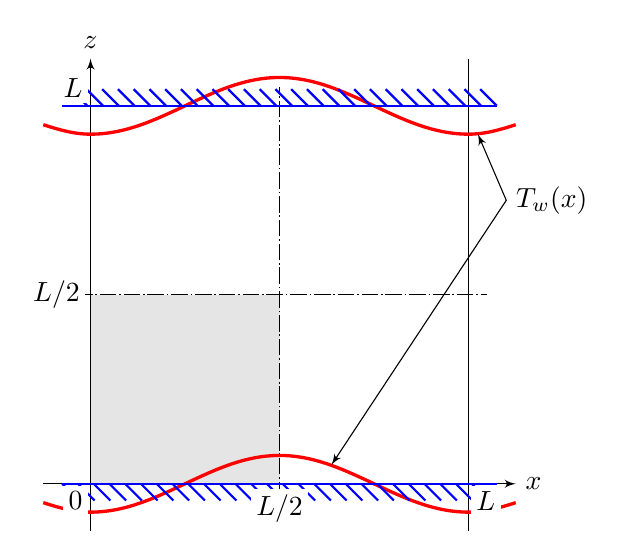
\begin{tikzpicture}[dashdot/.style={dash pattern=on .6pt off 1pt on 6pt off 1pt},
				interface/.style={postaction={draw, decorate, decoration=
					{border, angle=-45, amplitude=0.3cm, segment length=2mm}}},
				label/.style={fill=white, inner sep=2pt},
				>=latex', scale=1.2]
		\fill[gray!20] (0,0) -- (2,0) -- (2,2) -- (0,2) -- cycle;
		\draw[->] (-.5,0) -- (4.5,0) node[right] {\(x\)};
		\draw[->](0,-.5) -- (0,4.5) node[above] {\(z\)};
		\draw(4,-.5) -- (4,4.5);
		\draw[dashdot] (-.2,2) -- (4.2,2);
		\draw[dashdot] (2,-.2) -- (2,4.2);
		\draw[red, very thick] (-.5,-.2) sin (0,-.3) cos (1,0) sin (2,.3) cos (3,0) sin (4,-.3) cos (4.5,-.2);
		\draw[red, very thick] (-.5,3.8) sin  (0,3.7) cos (1,4) sin (2,4.3) cos (3,4) sin (4,3.7) cos (4.5,3.8);
		\draw[blue, thick, interface](-.3,0) -- (4.3,0);
		\draw[blue, thick, interface](4.3,4) -- (-0.3,4);
		\draw[<->] (4.1,3.7) -- (4.4,3) node[right] {\(T_w(x)\)} -- (2.55,.2);
		\node at (-.02,-.02) [below left, label] {0};
		\node at (4.02,-.02) [below right, label] {\(L\)};
		\node at (-.02,4.02) [above left, label] {\(L\)};
		\node at (-.05,2) [left, label] {\(L/2\)};
		\node at (2,-.05) [below, label] {\(L/2\)};
	\end{tikzpicture}
	\vspace{-20pt}
	\caption{Геометрия задачи.}\label{pic:geometry}
	\vspace{-10pt}
\end{wrapfigure}

\section{Решение задачи в гидродинамическом пределе}

\section{Решение для произвольных чисел Кнудсена}

\section{Сравнение результатов}

\end{document}


